%	DOCUMENT TYPE
%\documentclass{revtex4-1}
%\documentclass[showkeys]{revtex4-1}
%\documentclass[aps,prb,preprint,linenumbers]{revtex4-1}
%\documentclass[aps,prb,reprint]{revtex4-1}
%\documentclass[aps,prl,preprint,linenumbers]{revtex4-1}
%\documentclass[aps,prl,reprint]{revtex4-1}

\documentclass[notitlepage,11pt,nofootinbib]{revtex4-1}
%\documentclass[aps, preprint, prb, linenumbers, showpacs]{revtex4-1}

%	PACKAGES
\usepackage[utf8]{inputenc}
\usepackage{amssymb,amsmath,esint,amsfonts,mathtools,dsfont,bm}
\usepackage[usenames,dvipsnames]{xcolor}
\usepackage[pdftex]{graphicx}
\usepackage[pdftex,plainpages=false,colorlinks=true,linkcolor=Red, citecolor=blue, urlcolor=blue]{hyperref}
\usepackage[most]{tcolorbox}
\usepackage{empheq}


%	FONT
% \usepackage[fullfamily,lf,minionint,openg,loosequotes]{MinionPro}
%\usepackage[T1]{fontenc}
%\usepackage{microtype}
%\usepackage{times}
%\usepackage{mathptmx}
%\usepackage{newtxtext,newtxmath}
% \usepackage{txfonts}

\renewcommand{\vec}[1]{\bm{\mathrm{#1}}}

%% tensor

% \usepackage{stackengine}\stackMath
% \def\lvec{{\rotatebox{180}{$\mkern+0mu\mathchar"017E$}}}
% \def\tensign{\smash{\stackon[-1.99pt]{\mkern-4mu\mathchar"017E}{\rotatebox{180}{$\mkern+0mu\mathchar"017E$}}}}
% \def\boldsymbol#1{\def\useanchorwidth{T}\stackon[-4.3pt]{#1}{\,\tensign}}







%	DOCUMENT
\begin{document}

\title{Transport Theory Cookbook for Cuprates}
\author{S. \surname{Verret}}
% \author{G. \surname{Grissonnanche}}
% \author{M. \surname{Dion}}
\affiliation{D\'epartement de physique, Universit\'e de Sherbrooke, Qu\'ebec, Canada  J1K 2R1}
\date{\today}
% \keywords{}

\begin{abstract}
This document is a pedagogical reference that summarizes the mathematical relations between electronic transport coefficients, and shows how to compute them in the semi-classical approximation. We start with Chamber's formula and give the steps and approximations needed to get back to the Drude formula, leading to many useful intermediate results in between. All transport coefficients ultimately depend on only two parameters: the carriers lifetime $\tau_{\vec k}$ and their dispersion $E(\vec k)$. The last section define such a dispersion and lifetime to evaluate baseline transport results in cuprates.
\end{abstract}

\maketitle
\vspace{-0.5cm}
\tableofcontents

\section{Conductivity tensors}
\noindent
Three conductivity tensors $L_{11}$, $L_{12}$, and $L_{22}$ suffice to determine all electronic transport coefficients. They are tensors because they express the relations between $x$,$y$,$z$ components of: the electric current~$\vec j_e$, the heat current~$\vec j_Q$, the electric field~$\vec E$, and the Temperature gradient~$\vec \nabla T$~\cite{ashcroft_solid_1976,arsenault_transport_2013}:
\begin{align}
\vec j_e &= L_{11}\ \vec E + L_{12}\ (-\vec \nabla T),\\
\vec j_Q &= L_{21}\ \vec E + L_{22}\ (-\vec \nabla T).
\end{align}
These tensors depend on temperature $T$ and magnetic field $\vec B$, satisfying the Onsager relations:
$L_{11}(\vec B) = L_{11}^{\top}(-\vec B)$, $L_{22}(\vec B) = L_{22}^{\top}(-\vec B)$, and
$L_{12}(\vec B) = -TL_{21}^{\top}(-\vec B)$. Since
the latter defines $L_{21}$ from $L_{12}$, we can disregard $L_{21}$. These tensors' components are usually written:
\begin{align}
[L_{11}]_{ij} &= \sigma_{ij},
\\
[L_{12}]_{ij} &= \alpha_{ij},
\\
[L_{22}]_{ij} &= \beta_{ij},
\end{align}
with $i,j$ denoting $x,y,z$. In almost all cases, these can be computed as energy integrals of the same energy function $\sigma_{ij}(\epsilon)$, which we view here as a \emph{density of conductivity}:
\begin{align}
\sigma_{ij}
&=
\int_{-\infty}^{\infty} d\epsilon
\Big(-\frac{\partial f(\epsilon)}{\partial \epsilon}\Big)\sigma_{ij}(\epsilon)
\label{sigma}
\\
\alpha_{ij}
&=
\int_{-\infty}^{\infty}d\epsilon
\bigg[\Big(-\frac{\partial f(\epsilon)}{\partial \epsilon}\Big)\frac{\epsilon}{T}\bigg]\frac{\sigma_{ij}(\epsilon)}{-e}
\label{alpha}
\\
\beta_{ij}
&=
\int_{-\infty}^{\infty}d\epsilon
\bigg[\Big(-\frac{\partial f(\epsilon)}{\partial \epsilon}\Big)\frac{\epsilon^2}{T}\bigg]\frac{\sigma_{ij}(\epsilon)}{e^2}
\label{beta}
\\
C_V
&=
\int_{-\infty}^{\infty}d\epsilon
\bigg[\Big(-\frac{\partial f(\epsilon)}{\partial \epsilon}\Big)\frac{\epsilon^2}{T}\bigg]N(\epsilon).
\label{Cv}
\end{align}
with $-e$ as the electron charge. The name ``density of conductivity'' for $\sigma_{ij}(\epsilon)$ is not standard. I chose it because, as seen above, the specific heat $C_V$ can be computed from an identical integral, but with the density of states $N(\epsilon)$ taking the place of this $\sigma_{ij}(\epsilon)$. In the integrals above, $\sigma_{ij}(\epsilon)$ is always weighted by the derivative of the Fermi-Dirac distribution~$f(\epsilon)$:
\begin{align}
f(\epsilon) = \frac{1}{e^{\epsilon/k_{B}T}+1}.
\end{align}
The various functions seen in the brackets of~\eqref{sigma},~\eqref{alpha},~\eqref{beta}, and~\eqref{Cv} are illustrated in Fig.~\ref{figure_fermi} for various temperature $T$. Here are useful identities regarding these functions:
\begin{align}
\frac{\partial f(\epsilon)}{\partial \epsilon}
= 
-\frac{T}{\epsilon}
\frac{\partial f(\epsilon)}{\partial T} = 
\frac{1}{4k_BT\cosh^{2}(\epsilon/2k_BT)}.
\end{align}
Such functions are non-zero only in a narrow window surrounding the Fermi level (at $\epsilon=0$ in our convention). This is why we often only care about the Fermi surface when studying transport. 
We can displace the Fermi energy by considering $\epsilon = E_{\vec k}-\mu$, where the chemical potential~$\mu$ controls the expected number of particles $n$ filling the band $E_{\vec k}$ (with hole doping $p=1-n$).

\begin{figure}
\centering
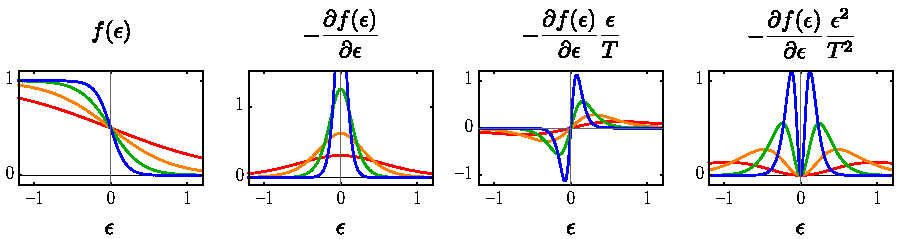
\includegraphics[width=\textwidth]{fermi.pdf}
\caption{Weighting functions involved in the expressions of transport coefficients, shown at temperatures $k_BT=0.8$ (red), $k_BT=0.4$ (orange), $k_BT=0.2$ (green), $k_BT=0.1$ (blue)}
\label{figure_fermi}
\end{figure}

Furthermore, at low temperature, expressions~\eqref{sigma},~\eqref{alpha},~\eqref{beta} and~\eqref{Cv} can all be approximated using the Sommerfeld expansion (see~\cite{ashcroft_solid_1976}, appendix C):
\begin{align}
\int_{-\infty}^{\infty} d\epsilon
\bigg(-\frac{\partial f(\epsilon)}{\partial \epsilon}\bigg)
K(\epsilon)
=
K(0)
+
\frac{\pi^2}{6}
k_{B}^2T^2
K''(0)
+
\frac{7\pi^4}{270}
k_{B}^2T^4
K''''(0)
+ \cdots
\end{align}
where primes denote the derivative. One can thus verify the following first order approximations:
\begin{align}
\sigma_{ij}
&\approx
\sigma_{ij}(0)
\label{sigma_expanded}
\\
\alpha_{ij}
&\approx
-\frac{\pi^2k_B^2 T}{3e}\sigma'_{ij}(0)
\label{alpha_expanded}
\\
\beta_{ij}
&\approx
-\frac{\pi^2k_B^2 T}{3e^2}\sigma_{ij}(0)
\label{beta_expanded}
\\
C_V
&\approx
-\frac{\pi^2k_B^2 T}{3}N(0)
\label{Cv_expanded}
\end{align}
where the Lorentz ratio $\frac{\pi^2k_B^2}{3e^2}$ links $\beta_{ij}/T$ and $\sigma_{ij}$ at low temperature (Wiedemann-Franz law).

The remaining sections of this document explain how to compute $\sigma_{ij}(\epsilon)$ in various limit of the semi-classical approximation. 
First, however, let us define the usual measurable transport coefficients (resistivity, Hall coefficient, Seebeck coefficient, etc.) in 2D, and give an example of how one can use the above formulation to think about those coefficients in cuprates, by comparing the resistivity and the Seebeck coefficient.

\subsection{Resistivity \& Hall effect}

The resistivity tensor $\boldsymbol{\rho}$ is defined as $L_{11}^{-1}$.
\begin{align}
\boldsymbol{\rho} &\equiv L_{11}^{-1}
=
\begin{pmatrix}
\sigma_{xx} & \sigma_{xy}\\
\sigma_{yx} & \sigma_{yy}
\end{pmatrix}^{-1}
=
\frac{1}{\sigma_{xx}\sigma_{yy}-\sigma_{xy}\sigma_{yx}}
\begin{pmatrix}
\sigma_{yy} & -\sigma_{xy}\\
-\sigma_{yx} & \sigma_{xx}
\end{pmatrix}
\end{align}
with longitudinal resistivity is then given as:
\begin{align}
\rho_{xx} 
&= 
\frac{\sigma_{yy}}{\sigma_{xx}\sigma_{yy} - \sigma_{xy}\sigma_{yx}}
\approx
\boxed{
\frac{1}{\sigma_{xx}}
},
\label{eq_resistivity}
\end{align}
where $\sigma_{xy}$ and $\sigma_{yx}$ are usually only non-zero under magnetic field $\vec B$, are usually very small, and give rise to the transverse resistivity:
\begin{align}
\rho_{xy} 
&= 
\frac{-\sigma_{xy}}{\sigma_{xx}\sigma_{yy} - \sigma_{xy}\sigma_{yx}},
\approx
\boxed{
\frac{-\sigma_{xy}}{\sigma_{xx}\sigma_{yy}}
}.
\end{align}
From the latter, the Hall coefficient, $R_H$ and the Hall number, $n_H$, are defined as:
\begin{align}
R_H = \frac{-\rho_{xy}}{B}
&\qquad
n_H = \frac{1}{-eR_H}.
\end{align}



\subsection{Thermoelectricity: Seebeck, Pelletier \& Nernst effects}

The thermoelectricity tensor $\boldsymbol{Q}$ is defined as:
\begin{align}
\boldsymbol{Q} &\equiv L_{11}^{-1}L_{12}
=
\begin{pmatrix}
\sigma_{xx} & \sigma_{xy}\\
\sigma_{yx} & \sigma_{yy}
\end{pmatrix}^{-1}
\begin{pmatrix}
\alpha_{xx} & \alpha_{xy}\\
\alpha_{yx} & \alpha_{yy}
\end{pmatrix}
=
\begin{pmatrix}
  \frac{\sigma_{yy}\alpha_{xx}-\sigma_{xy}\alpha_{yx}}
  {\sigma_{xx}\sigma_{yy}-\sigma_{xy}\sigma_{yx}} 
& \frac{\sigma_{yy}\alpha_{xy}-\sigma_{xy}\alpha_{yy}}
  {\sigma_{xx}\sigma_{yy}-\sigma_{xy}\sigma_{yx}}\\
  \frac{\sigma_{xx}\alpha_{yx}-\sigma_{yx}\alpha_{xx}}
  {\sigma_{xx}\sigma_{yy}-\sigma_{xy}\sigma_{yx}}
& \frac{\sigma_{xx}\alpha_{xy}-\sigma_{yx}\alpha_{yy}}
  {\sigma_{xx}\sigma_{yy}-\sigma_{xy}\sigma_{yx}}
\end{pmatrix}
\end{align}
Therefore, the Seebeck coefficient corresponds to
\begin{align}
S_x
\equiv 
Q_{xx} 
=
\frac{\sigma_{yy}\alpha_{xx}-\sigma_{xy}\alpha_{yx}}{\sigma_{xx}\sigma_{yy}-\sigma_{xy}\sigma_{yx}} 
\approx 
\boxed{
\frac{\alpha_{xx}}{\sigma_{xx}}
}.
\label{eq_seebeck}
\end{align}
for which first order Sommerfeld approximations~\eqref{sigma_expanded} and~\eqref{alpha_expanded} lead to the Mott formula:
\begin{align}
S_x = \frac{\alpha_{xx}}{\sigma_{xx}} 
&= - \frac{\pi^2 k_B^2 T}{3e}\frac{ \sigma'_{xx}(0)}{ \sigma_{xx}(0)}
\\
\Aboxed{
S_x
& = - \frac{\pi^2 k_B^2 T}{3e}\frac{\partial \log \sigma_{xx}(\epsilon) }{\partial \epsilon}\Big\vert_{\epsilon=0}
},
\end{align}
The Nernst coefficient is givent by:
\begin{align}
N 
\equiv
Q_{xy}
&= 
\frac{\sigma_{yy}\alpha_{xy}-\sigma_{xy}\alpha_{yy}}
{\sigma_{xx}\sigma_{yy}-\sigma_{xy}\sigma_{yx}}
\approx 
\boxed{
\frac{\alpha_{xy}}{\sigma_{xx}}
- S_{y}\frac{\sigma_{xy}}{\sigma_{xx}}
}
\end{align}

\subsection{Thermal conductivity \& Righi-Leduc effect}
In the same way, the thermal conductivity $\boldsymbol{\kappa}$ can be obtained from:
\begin{align}
\boldsymbol{\kappa} &\equiv L_{22} - TL_{12}L_{11}^{-1}L_{12}
\end{align}
which yields thermal conductivity:
\begin{align}
\kappa_{xx} 
&=
T\Big(\frac{
\alpha_{xx}\sigma_{yy}\alpha_{xx} -
\alpha_{xx}\sigma_{xy}\alpha_{yx} -
\alpha_{xy}\sigma_{yx}\alpha_{xx} +
\alpha_{xy}\sigma_{xx}\alpha_{yx}
}{\sigma_{xx}\sigma_{yy}-\sigma_{xy}\sigma_{yx}}
\Big) - \beta_{xx}
\\ &
\approx
T
% \Big( 
\frac{
\alpha_{xx}^2
}{\sigma_{xx}}
% +
% \frac{
% \alpha_{xy}\alpha_{yx}
% }{\sigma_{yy}}
% \Big)
- \beta_{xx}
\end{align}
and the Righi-Leduc (or thermal Hall) coefficient:
\begin{align}
\kappa_{xy} 
&=
T\Big(\frac{
\alpha_{xx}\sigma_{yy}\alpha_{xy} -
\alpha_{xx}\sigma_{xy}\alpha_{yy} -
\alpha_{xy}\sigma_{yx}\alpha_{xy} +
\alpha_{xy}\sigma_{xx}\alpha_{yy}
}{\sigma_{xx}\sigma_{yy}-\sigma_{xy}\sigma_{yx}}
\Big) - \beta_{xy}
\\ &
\approx
T\Big( \frac{
\alpha_{xx}\alpha_{xy}
}{\sigma_{xx}}
+
\frac{
\alpha_{xy}\alpha_{yy}
}{\sigma_{yy}}
\Big) - \beta_{xy}
\end{align}

\subsection{Example of interpretation for the Seebeck effect}
When substituting the expressions the resistivity \eqref{eq_resistivity} for $\rho_{xx}$ and \eqref{alpha} for $\alpha_{xx}$ in the reduced expression for the Seebeck coefficient~\eqref{eq_seebeck}, one gets a particularily revealing expression regarding the density of conductivity $\sigma_{xx}(\epsilon)$:
\begin{align}
S_x 
&=
\frac{\alpha_{xx}}{\sigma_{xx}}
=
\frac{\rho_{xx}}{-eT}
\int_{-\infty}^{\infty}d\epsilon
\Big(-\frac{\partial f(\epsilon)}{\partial \epsilon}\Big)
\ \epsilon\ 
\sigma_{xx}(\epsilon).
\label{eq_seebeck_explicit}
\end{align}
In this expression, we can see that if $\sigma_{xx}(\epsilon)$ is even with respect to the Fermi-level, \emph{i.e.} $\sigma_{xx}(-\epsilon) = \sigma_{xx}(\epsilon)$ within the narrow energy window determined by $-\frac{\partial f(\epsilon)}{\partial \epsilon}$, then, because of the extra $\epsilon$ in the integral, the integrand is perfectly odd and the Seebeck coefficient should be zero. Thus, any non-zero Seebeck effect must come from an assymetry in the density of conductivity $\sigma_{xx}(\epsilon)$ with respect to the Fermi level.

Equation~\ref{eq_seebeck_explicit} is particularily relevant to cuprates, regarding the pseudogap transition occuring at doping~$p^*$. At low temperature, an abrupt augmentation of the resistivity~$\rho_{xx}$ is observed at~$p^*$. Since resistivity explicitely enters expression~\eqref{eq_seebeck_explicit}, an equivalent augmentation is expected in the Seebeck effect, given the latter is non-zero. However, a comparison between the augmentation in $\rho_{xx}$ and the augmentation in $S_x$ might reveal a lot more. Namely, if the $p^*$ transition causes $\sigma_{xx}(\epsilon)$ to change symetrically in energy with respect to the Fermi level, then the only effect in $S_x$ will come from $\rho_{xx}$, because the $\epsilon$ would make the symmetric changes of the transition an odd contribution in the integral of~\eqref{eq_seebeck_explicit}, which would cancel out. In that case, the Seebeck augmentation should track the resistivity augmentation exactly. On the other hand, if the change in $\sigma_{xx}(\epsilon)$ is assymetric with respect to the Fermi level, then there will be a difference between the augmentations in $S_x$ and that in $\rho_{xx}$. Note that in either cases, the Seebeck effect can remain nonzero at all times, given a sufficiently assymetric $\sigma_{xx}(\epsilon)$; only the eveness or oddness of \emph{the changes} brought by the transition are relevant.

\subsection{Note on the strongly correlated case}

The above analysis remains mostly valid in the strongly correlated case. As we we will see in the next section, the non-interacting, zero-field $\sigma_{xx}(\epsilon)$ is:
\begin{align}
\sigma_{xx}(\epsilon)
&=
e^2\iiint_{\text{BZ}}\frac{d^3k}{(2\pi)^3}
v_{x}(\vec k)^2
\tau_{\vec k}\delta\big(\epsilon-E(\vec k)\big),
\label{eq_will_return}
\end{align}
In the strongly correlated case, $\sigma_{xx}(\epsilon)$ would be the current-current correlation function, given in first approximation by:
\begin{align}
\sigma_{xx}(\epsilon) 
&=
e^2\iiint_{\text{BZ}}\frac{d^3k}{(2\pi)^3}
v_{x}(\vec k)^2
\pi\hbar A(\vec k,\epsilon)^2,
\end{align}
where $A(\vec k,\epsilon)$ is the spectral weight.

The above correspondence for the longitudinal conductivity has an analogous one for the transverse conductivity (not shown here, please refer to~\cite{verret_phenomenological_2017}). These correspondance between non-interacting and interacting transport functions suggests the following heuristic:
\begin{align}
\tau_{\vec k}\delta\big(\epsilon-E(\vec k)\big) &\longleftrightarrow \pi\hbar A(\vec k,\epsilon)^2
\\
\tau_{\vec k}^2\delta\big(\epsilon-E(\vec k)\big) &\longleftrightarrow \frac{\pi^2\hbar^2}{3} A(\vec k,\epsilon)^3
\label{tauSquare}
\end{align}
to go from one to the other. This might be useful to guide more rigorous derivation of strongly correlated formulas. Note that expressions such as~\eqref{tauSquare} only consider linear order in magnetic field (section~\ref{sec_zeroField}) and neglect vertex corrections.

\section{Complete Semi-classical formulas}
\noindent
To get full magnetic field dependence in $\sigma_{ij}(\epsilon)$, one must use the Chambers Formula~\cite{ashcroft_solid_1976}:
\begin{align}
\sigma_{ij}(\epsilon) 
&=
e^2\iiint_{\text{BZ}}\frac{d^3k}{(2\pi)^3}
v_{i}(\vec k)\bar{v}_{j}(\vec k)
\delta\big(\epsilon-E(\vec k)\big),
\label{chambers1}
\end{align}
which is an integral on all $\vec k$-states in the first Brillouin zone (BZ). The Dirac delta indicates that each states only contributes to this ``density of conductivity'' at the energy~$E(\vec k)$. The weight of this contribution is given by a component of the group velocity~$\vec v(\vec k)$:
\begin{align}
v_{i}(\vec k) = \frac{1}{\hbar}\frac{\partial E(\vec k)}{\partial k_i},
\label{velocity}
\end{align}
multiplied by a ``decaying'' or ``travelling'' velocity, $\bar{v}_{j}(\vec k)$:
\begin{align}
\bar{v}_{j}(\vec k)
&=
\int_{0}^{\infty}dt
\exp\Big[
-\int_{0}^{t}dt'/\tau_{\vec k(t')}
\Big]
v_{j}(\vec k(t)),
\label{chambers2}
\end{align}
where we find the lifetime $\tau_{\vec k}$ (which is not only $\vec k$-dependent, but can also be $\epsilon$- and $T$-dependent, as discussed in section~\ref{section_lifetime}). Both $\tau_{\vec k}$ and $v_j(\vec k)$ are evaluated on a trajectory $\vec k(t)$, in $\vec k$-space. This trajectory starts at $\vec k(0)=\vec k$, and is governed by the semiclassical equation of motion:
\begin{align}
\hbar\frac{d\vec k(t)}{dt} =
-e \big(\vec v(\vec k(t))\times\vec B \big)
\label{semiClassicalMovement}
\end{align}
where $\vec B$ is the magnetic field. To compute conductivity tensors, one must thus solve this differential equation \eqref{semiClassicalMovement} for each starting point $\vec k$ contained the integral of \eqref{chambers1}.

\begin{tcolorbox}[colback=black!2!white,colframe=white!10!black,title=All-in-one equation]
We can reduce all the tensors into a single expression. We substitute \eqref{chambers2} and \eqref{velocity} in \eqref{chambers1}, and then substitute the result in \eqref{sigma}, \eqref{alpha}, and \eqref{beta}, unifying them in the following monster:
\begin{align}
\sigma_{ij}^{(n)}
&=
\int_{-\infty}^{\infty}d\epsilon
\bigg[\Big(-\frac{\partial f(\epsilon)}{\partial \epsilon}\Big)\frac{\epsilon^{n}}{T^{n}}\bigg]
(-e)^{2-n}\iiint_{\text{BZ}}\frac{d^3k}{(2\pi)^3}
\frac{1}{\hbar}\frac{\partial E(\vec k)}{\partial k_i} %v_{i}(\vec k)
\nonumber\\
&\qquad\times
\int_{0}^{\infty}dt
\exp\Big[
-\int_{0}^{t}dt'/\tau_{\vec k(t')}
\Big]
\frac{1}{\hbar}\frac{\partial E(\vec k)}{\partial k_j}\Big|_{\vec k(t)} %v_{j}(\vec k(t))
\ \delta\big(\epsilon-E(\vec k)\big)
\label{chambers}
\end{align}
with:
\begin{align}
\sigma_{ij}&=\sigma_{ij}^{(0)}\\
\alpha_{ij}&=\sigma_{ij}^{(1)}\\
\frac{\beta_{ij}}{T}&=\sigma_{ij}^{(2)}.
\end{align}
The semiclassical movement equation \eqref{semiClassicalMovement} must be used to find $\vec k(t)$. The only free paramters associated to the material under study are $E(\vec k)$ and $\tau_{\vec k}$. 
\end{tcolorbox}






\section{Simplifications}


\subsection{Equi-energy surfaces}\label{sec_surfaces}
The Dirac delta $\delta(\epsilon-E(\vec k))$ allow to change the three-dimensional $\vec k$ integral to a two-dimensional integral on the surface defined by $E(\vec k)=\epsilon$ (see equation~8.57 and 8.62 of Ashcroft~\&~Mermin~\cite{ashcroft_solid_1976} for a similar statement).
Indeed, for arbitrary $F(\vec k)$, we can rewrite the integral as:
\begin{align}
\iiint d^3 k 
F(\vec k)\delta\big(\epsilon - E(\vec k)\big)
&=
\iint d^2k_{\parallel}
\int dk_{\perp}
F(\vec k)\delta\big(\epsilon - E(\vec k)\big),
\end{align}
where a change of variable was used at each point of space, to the basis where $k_{\perp}$ is the component of $\vec k$ perpendicular to the surface defined by $E(\vec k)=\epsilon$, and $k_{\parallel}$ are the two components parallel to this surface. In this new basis, an infinitesimal change of $\epsilon$ is always along $k_{\perp}$
\begin{align}
\epsilon + d\epsilon &= \epsilon + |\nabla_{\vec k}E(\vec k)|dk_{\perp}
\end{align}
so the $\delta(\epsilon - E(\vec k))$ allows to remove the integral on $k_{\perp}$: 
\begin{align}
\iiint d^3 k 
F(\vec k)\delta\big(\epsilon - E(\vec k)\big)
% &=
% \iint d^2k_{\parallel} 
% \int \frac{d\epsilon}{|\nabla_{\vec k}E(\vec k)|}
% F(\vec k)\delta\big(\epsilon - E(\vec k)\big)
% \\
&=
\iint d^2k_{\parallel} 
\frac{F(\vec k)}{|\nabla_{\vec k}E(\vec k)|}.
% \intertext{Question: could this be written as}
% \delta\big(\epsilon-E(\vec k)\big)
% &=
% \iint d^2 k \frac{\delta^{3}(\vec k-\vec k)}{|\vec \nabla_{\vec k} E(\vec k)|_{\vec k=\vec k}}\ ?
\end{align}
Although it seems to have disapear, the dependence in $\epsilon$ still exists implicitely in the bounds of the integral: the $k_{\parallel}$ run along the surface defined by $E(\vec k)=\epsilon$.

The above allow to rewrite \eqref{chambers1} as:
\begin{align}
\Aboxed{
\sigma_{ij}(\epsilon) 
&=
e^2
\iint\limits_{\substack{E(\vec k)=\epsilon\\ \text{in BZ}}}
\frac{d^2k_{\parallel}}{(2\pi)^3}
\frac{v_{i}(\vec k)\bar{v}_{j}(\vec k)}{\hbar|\vec v(\vec k)|}
}.
\label{chambersSurfaces}
\end{align}

\subsection{Zero Magnetic field}\label{sec_zeroField}
In the limit of zero magnetic field, $\vec B\rightarrow0$, the differential equation \eqref{semiClassicalMovement} becomes trivial, and $\vec k (t)=\vec k$ at all $t$. In that case, \eqref{chambers2} simply reduces to:
\begin{align}
\bar{v}_{j}(\vec k)
&=
v_{j}(\vec k)
\int_{0}^{\infty}dt
e^{-t/\tau_{\vec k}}
\\
&=
v_{j}(\vec k)
\tau_{\vec k}.
\end{align}
However, in the case of $i\neq j$, $\sigma_{ij}(\omega)$ is zero at zero field, so we shall keep the linear term in $\vec B$ in this case (see~\cite{ziman_electrons_1960} for details). This allows to write \eqref{chambers1} as:
\begin{empheq}[box=\fbox]{align}
\lim_{\vec B\rightarrow0}\sigma_{ij}(\epsilon) 
&=
e^2\iiint_{\text{BZ}}\frac{d^3k}{(2\pi)^3}
\Bigg[
\delta_{ij}
v_{i}(\vec k)
v_{i}(\vec k)
\tau_{\vec k}
\delta\big(\epsilon-E(\vec k)\big)
\nonumber\\
&
% \phantom{=\iiint_{\text{BZ}}\frac{d^3k}{(2\pi)^3}}
\qquad\qquad\qquad
% -\varepsilon_{ijk}(-eB_{k})
+e\varepsilon_{ijk}B_{k}
\Big[
v_{i}(\vec k)
v_{i}(\vec k)
\frac{\partial v_{j}(\vec k)}{\partial k_j}
-
v_{i}(\vec k)
v_{j}(\vec k)
\frac{\partial v_{i}(\vec k)}{\partial k_j}
\Big]
\tau_{\vec k}^2
\delta\big(\epsilon-E(\vec k)\big)
\Bigg],
\label{chambersZeroField}
\end{empheq}
where $\delta_{ij}$ is the Kronecker symbol and $\varepsilon_{ijk}$ is the Levi-Cevita symbol (which is 0 if $i=j$). The first term of this equation thus corresponds to~\eqref{eq_will_return}.

\subsection{Effective mass and Drude results}

We can carry out explicitely the integral over energy in the all-in-one equation~\eqref{chambers} and reorganize it as: 
\begin{align}
\sigma_{ij}^{(n)}
&=
-\frac{(-e)^{2-n}}{\hbar T^n}
% \int_{0}^{\infty}dt
% e^{-\int_{0}^{t}dt'/\tau_{\vec k(t')}}
\iiint_{\text{BZ}}\frac{d^3k}{(2\pi)^3}
E(\vec k)^{n}
\frac{\partial f(\epsilon)}{\partial E(\vec k)}
\frac{\partial E(\vec k)}{\partial k_i}
% \frac{\partial E(\vec k(t))}{\partial k_j}
\bar{v}_j(\vec k)
\\
&=
-\frac{(-e)^{2-n}}{\hbar T^n}
% \int_{0}^{\infty}dt
% e^{-\int_{0}^{t}dt'/\tau_{\vec k(t')}}
\iiint_{\text{BZ}}\frac{d^3k}{(2\pi)^3}
E(\vec k)^{n}
\frac{\partial f(E(\vec k))}{\partial k_i}
% \frac{\partial E(\vec k(t))}{\partial k_j}
\bar{v}_j(\vec k).
\label{checkPointMass}
\end{align}
This allow to integrate by parts as follows:
\begin{align}
\int_{-\pi/a_i}^{\pi/a_i} dk_i\ 
E(\vec k)^{n}
\frac{\partial
f(E(\vec k))
}{\partial k_i}
% \frac{\partial E(\vec k(t))}{\partial k_j}
\bar{v}_j(\vec k)
&=
\bigg[
E(\vec k)^{n}
f(E(\vec k))
% \frac{\partial E(\vec k(t))}{\partial k_j}
\bar{v}_j(\vec k)
\bigg]_{-\pi/a_i}^{\pi/a_i}
\nonumber\\
&\quad-
\int_{-\pi/a_i}^{\pi/a_i} dk_i\ 
nE(\vec k)^{n-1}
\frac{\partial E(\vec k)}{\partial k_i}
f(E(\vec k))
% \frac{\partial E(\vec k(t))}{\partial k_j}
\bar{v}_j(\vec k)
\nonumber\\
&\quad-
\int_{-\pi/a_i}^{\pi/a_i} dk_i\ 
E(\vec k)^{n}
f(E(\vec k))
% \frac{\partial^2 E(\vec k(t))}{\partial k_i\partial k_j}
\frac{\partial\bar{v}_j(\vec k)}{\partial k_i}.
\label{integrationBy3Parts}
\end{align}
Since $n$ only takes the values $0,1,2$, and under the conditions $E(-\vec k)=E(\vec k)$,
and $\bar{v}_j(-\vec k)$ = $-\bar{v}_j(\vec k)$, then the first and second terms of \eqref{integrationBy3Parts} are zero, and \eqref{checkPointMass} becomes:
\begin{align}
\Aboxed{
\sigma_{ij}^{(n)}
&=
(-e)^{2-n}
% \int_{0}^{\infty}dt
% e^{-\int_{0}^{t}dt'/\tau_{\vec k(t')}}
\iiint_{\text{BZ}}\frac{d^3k}{(2\pi)^3}
\frac{E(\vec k)^{n}}{T^n}
% \frac{\partial^2 E(\vec k(t))}{\partial k_i\partial k_j}
\frac{1}{\hbar}
\frac{\partial\bar{v}_j(\vec k)}{\partial k_i}
f(E(\vec k))
}.
\end{align}
Taking explicitely the derivative of \eqref{chambers2}:
\begin{align}
\frac{1}{\hbar}\frac{\partial\bar{v}_j(\vec k)}{\partial k_i}
&=
\int_{0}^{\infty}dt\ 
\bigg[
e^{-\int_{0}^{t}dt'/\tau_{\vec k(t')}}
\frac{1}{\hbar^2}\frac{\partial^2 E(\vec k(t))}{\partial k_i\partial k_j}
\nonumber\\
&\qquad\qquad+
e^{-\int_{0}^{t}dt'/\tau_{\vec k(t')}}
\Big(
\int_{0}^{t}\frac{dt'}{\tau_{\vec k(t')}^2}
\frac{\partial\tau_{\vec k(t')}}{\partial k_i}
\Big)
\frac{1}{\hbar^2}\frac{\partial E(\vec k(t))}{\partial k_j}
\bigg]
\label{eq_velocity_derivative}
\end{align}
we find the effective mass:
\begin{align}
M^{-1}_{ij}(\vec k)
\equiv
\frac{1}{\hbar^2}\frac{\partial^2 E(\vec k)}{\partial k_i\partial k_j}.
\label{effectiveMass}
\end{align}
Note that if the lifetime is independent of $\vec k$, then the second term of~\eqref{eq_velocity_derivative} disappears, and only the first term remains. In that case, carrying the zero magnetic field manipulations of \ref{sec_zeroField} and restituting of the integral in energy lead to:
\begin{empheq}[box=\fbox]{align}
\lim_{\substack{\vec B\rightarrow 0\\ \tau_{\vec k}\rightarrow\tau}}
\sigma_{ij}^{(n)}
&=
\int_{-\infty}^{\infty}
d\epsilon
f(\epsilon)
\frac{\epsilon^{n}}{T^n}
(-e)^{2-n}
% \int_{0}^{\infty}dt
% e^{-\int_{0}^{t}dt'/\tau_{\vec k(t')}}
\iiint_{\text{BZ}}\frac{d^3k}{(2\pi)^3}
% \frac{\partial^2 E(\vec k(t))}{\partial k_i\partial k_j}
\Bigg[
\delta_{ij}M^{-1}_{ii}(\vec k)\tau
\nonumber\\
&\qquad
+\varepsilon_{ijk}(-eB_k) \bigg(M^{-1}_{ii}(\vec k)M^{-1}_{jj}(\vec k) - \big( M^{-1}_{ij}(\vec k) \big)^2 \bigg)\tau^2
\Bigg]
\delta(\epsilon-E(\vec k))
,
\end{empheq}
The above is an all-in-one equation expressed with the mass instead of the velocities.
Note in particular the longitudinal electric conductivity case $\sigma_{ii} = \sigma_{ii}^{(0)}$:
\begin{align}
\lim_{\substack{\vec B\rightarrow 0\\ \tau_{\vec k}\rightarrow\tau}}
\sigma_{ii}
&=
\iiint_{\text{BZ}}\frac{d^3k}{(2\pi)^3}
f(E(\vec k))
e^2
M^{-1}_{ii}(\vec k)
\tau_{\vec k},
\end{align}
which reduces to the Drude formula when $M_{ij}^{-1}(\vec k) = \delta_{i,j}\frac{1}{m^*_i}$:
\begin{align}
\Aboxed{
\lim_{\substack{
\vec B\rightarrow 0, 
\tau_{\vec k}\rightarrow\tau\\
M_{ij}(\vec k)\rightarrow \delta_{ij}m^*_i
}}
\sigma_{ij}
&=
\delta_{i,j}
\frac{ne^2\tau}{m^*_i}
}
\end{align}



\subsection{Zero temperature}
In the zero temperature limit, the electrical conductivity tensor \eqref{sigma} becomes: 
\begin{align}
\lim_{T\rightarrow 0}\sigma_{ij}
&=
\int_{-\infty}^{\infty} d\epsilon
\lim_{T\rightarrow 0}\Big(-\frac{\partial f(\epsilon)}{\partial\epsilon}\Big) \sigma_{ij}(\epsilon)
\\
&=
\int_{-\infty}^{\infty} d\epsilon
\delta(\epsilon-\mu) \sigma_{ij}(\epsilon)
\\
\Aboxed{
\lim_{T\rightarrow 0}\sigma_{ij}&=\sigma_{ij}(\mu).
}
\end{align}
Unfortunately, this simplification does not extend to $\alpha_{ij}$ and $\beta_{ij}$ for which one must instead turn to Sommerfeld expansions (very well explained at Appendix~C of Ashcroft~\&~Mermin~\cite{ashcroft_solid_1976}).
Note that together with the simplification \ref{sec_surfaces} for energy surfaces, the zero-temperature simplification implies that the conductivity at $T=0$ is entirely given by the Fermi Surface:
\begin{align}
\lim_{T\rightarrow0}\sigma_{ij} 
=\frac{e^2}{(2\pi)^3}\iint_{\text{FS}}d^2k_F
\frac{v_{i}(\vec k_F)\bar{v}_{j}(\vec k_F)}{\hbar|\vec v(\vec k_F)|}.
\label{zeroTemperature}
\end{align}



\section{For cuprates}\label{section_disp}
\noindent
When working with cuprates, we consider two candidates for $E(\vec k)$: (i) the bare dispersion $\epsilon_{\text{3D}}(\vec k)$, and (ii) the antiferromagnetic approximation for the pseudogap $E^{\pm}_{\text{3D}}(\vec k)$. Both are introduced in what follow.

\subsection{Bare dispersion}\label{section_doping}
To simulate overdoped cuprates, we use the one-band three-dimensional dispersion measured by ARPES~\cite{horio_three-dimensional_2018} in Eu-LSCO:
\begin{align}
\epsilon_{\text{3D}}(\vec k)=\epsilon_{\vec k}+\epsilon_{\perp}(\vec k)
\end{align}
where $\epsilon_{\vec k}$ is the plane dispersion:
\begin{align}
\epsilon_{\vec k} 
&= 
-2t\big(\cos (k_xa) + \cos (k_yb)\big)
% \nonumber\\
% &\phantom{=\ }
-4t'\cos (k_xa)\cos (k_yb)
% \nonumber\\
% &\phantom{=\ }
-2t''\big(\cos (2k_xa)+\cos (2k_yb)\big)
\end{align}
and $\epsilon_{\perp}(\vec k)$ is the inter-plane dispersion:
\begin{align}
\epsilon_{\perp}(\vec k)
&=
-2t_z\cos\Big(\frac{k_xa}{2}\Big)
\cos\Big(\frac{k_yb}{2}\Big)
\cos\Big(\frac{k_zc}{2}\Big)
% \nonumber\\
% &\phantom{=\ }\times
\big(\cos (k_xa) - \cos (k_yb)\big)^2.
\end{align}
We use parameters $a=b=3.75$ {\AA}, $c=13.20$ {\AA}, $t=190$ meV, and $(t',t'',t_z)=(-0.14t,0.07t,0.07t)$. The chemical potential $\mu$ is obtained by solving the integral equation for a given doping $p$:
\begin{align}
p &= 1 - n \\
&= 1 - \iiint_{BZ} \frac{d^{3}k}{4\pi^{3}} f(\epsilon_{\text{3D}}(\vec k)-\mu)
\end{align}

\subsection{Approximation for the pseudogap} 
To fit the results for the pseudogap regime at $p<p^*$, we start from a two-dimensional antiferromagnetic (AF) reconstruction of the bare band (following recent success of such a model for the Hall number~\cite{storey_hall_2016,verret_phenomenological_2017}):
\begin{align}
E^{\pm}(\vec k) 
= 
\tfrac{1}{2}(\epsilon_{\vec k}+\epsilon_{\vec k+\vec Q})
\pm \sqrt{
\tfrac{1}{4}(\epsilon_{\vec k}-\epsilon_{\vec k+\vec Q})^2 + M^2}
\end{align}
We cannot extend this model straightforwardly to the three-dimensional dispersion, because taking $\epsilon_{\vec k}\rightarrow\epsilon_{\text{3D}}(\vec k)$ in the above equation results in C4 rotational symmetry breaking. This is because of the body-centered structure of Nd-LSCO, which is fully taken into account in $\epsilon_\perp(\vec k)$, and in for which antiferromagnetism is not the same for $\vec Q=(\pi/a,\pi/a,0)$ than for $\vec Q=(\pi/a,-\pi/a,0)$. Therefore, we can instead suppose that the 2D planes contain independent antiferromagnetic orders, and add the $z$-dispersion after the reconstruction:  
\begin{align}
E^{\pm}_{\text{3D}}(\vec k)=E^{\pm}(\vec k)+\epsilon_{\perp}(\vec k)
\end{align}
This may be interpreted as antiferromagnetism uncorrelated between planes.

\paragraph*{Note on numerical optimization:}
The bottleneck when evaluating equations~\eqref{zeroTemperature} at zero temperature or~\eqref{chambersSurfaces} at finite temperature is the repeated evaluation of the velocity required to solve the semiclassical equation~\eqref{semiClassicalMovement}. In practice, we can save a lot of computation time by noting that $\epsilon_{\vec k+\vec Q}$ and $\vec v(\vec k+\vec Q)$ are simply linked to $\epsilon_{\vec k}$. We first split the latter as:
\begin{align}
\epsilon_{\vec k} &= \zeta_{\vec k} + \xi_{\vec k}
\\
\xi_{\vec k}
&\equiv
-2t\big(\cos (k_xa) + \cos (k_yb)\big),
\\
\zeta_{\vec k} 
&\equiv
-4t'\cos (k_xa)\cos (k_yb)
\nonumber \\
&\phantom{=\ }
-2t''\big(\cos (2k_xa)+\cos (2k_yb)\big)
\end{align}
and note that for $\vec Q=(\pi/a,\pi/a)$:
\begin{align}
\epsilon_{\vec k+\vec Q} &= \zeta_{\vec k} - \xi_{\vec k}
\end{align}

\subsection{Lifetime}\label{section_lifetime}

The various lifetime $\tau_{\vec k}$ we consider are those of previous work on Hall and Seebeck effets~\cite{verret_phenomenological_2017}, and those of the review by Hussey~\cite{hussey_phenomenology_2008}. The lifetime is the inverse of the total scattering rate:
\begin{align}
\tau_{\vec k}=\frac{\hbar}{2\Gamma(\vec k)},
\end{align}
and the scattering rate can have various contributions:
\begin{align}
\Gamma(\vec k,\omega,T) 
&=\eta_0
+ \eta_{1}\omega
+ \eta_{\ell}|\vec v(\vec k)|
+ \eta_{N}/|\vec v(\vec k)|
\nonumber\\&
\phantom{=\ }
+ \eta_{\text{PL}}T
+ \eta_{\text{FL}_a}(\omega^2 + \pi^2T^2)
% \nonumber\\&
% \phantom{=\ }
+ \eta_{\text{FL}_b}(\omega^2 + \pi^2T^2)/|\vec v(\vec k)|
\nonumber\\&
\phantom{=\ }
+ (\eta_{\text{an}} + \eta_{\text{an}1}\omega)\big(\cos k_x - \cos k_y\big)^{12}
\end{align}
In this expression, a small non-zero value for $\eta_0$ is usually needed to prevent divergence. Taken alone, $\eta_0$ would yield constant lifetime, $\eta_\ell$ would yield constant mean-free path, $\eta_N$ would yield scattering proportional to the density of state, $\eta_1$ provides a linear dependence in energy (allows to control the sign of $\alpha$ to some extent), $\eta_{\text{FL}_a}$ gives a Fermi-Liquid dependence, $\eta_{\text{FL}_b}$ a Fermi liquid dependence proportional to the density of states and $\eta_{\text{an}}$ yields a phenomenological increase of the anti-nodal scattering and $\eta_{\text{an}1}$ extends the linear energy dependence to this anisotropy. There can be various reasons to consider each terms separately, or combined or to add new terms.

% \section{strongly correlated case}

% Please refer to Arsenault \emph{et al.}~\cite{arsenault_transport_2013}  for the strongly correlated case. Note that the analysis for equation 

% \begin{acknowledgments}
% Most of the work that lead to this note was done with Gaël Grissonanche, closely following the work of Pr. Brad Ramshaw and Yawen Fang in Cornell University.
% \end{acknowledgments}


\bibliography{cookbook}

\end{document}

